%----------------------------------------------------------------------------------------
% CHAPTER THREE
%----------------------------------------------------------------------------------------
\chapter{THZ-INDUCED HHG AND NONLINEWAR CHARGE TRANSPORT \label{ch:ch4}}

Researchers have probed HHG in graphene particularly within the terahertz (THz) regime \cite{hafez2018extremely,kovalev2021electrical}. THz-induced transparency of graphene, an intriguing nonlinear optical effect, has been explored \cite{Hwang2013,Paul_2013,doi:10.1063/1.4902999}, often analyzed through a thermodynamic model emphasizing the reduction of electric conductivity \cite{mics2015thermodynamic,kovalev2021electrical}.
Despite these advancements, a comprehensive understanding of the microscopic mechanisms governing these nonlinear effects remains elusive. The existing studies predominantly rely on thermodynamic models, lacking a thorough exploration of nonequilibrium quantum dynamics under dissipation. This research gap highlights the need for a deeper exploration of the underlying microscopic processes to unravel the intricacies of HHG and related nonlinear optical effects in graphene.

In this chapter, we delve into the intricate details of terahertz (THz)-induced high-order harmonic generation (HHG) and nonlinear electric transport in graphene. Our approach involves utilizing the quantum master equation with the relaxation time approximation to provide a comprehensive understanding of the underlying phenomena. To gain microscopic insights, we meticulously compare the outcomes of fully dynamic calculations with those obtained through a quasi-static approximation, wherein the electronic system is treated as a nonequilibrium steady state.

The key revelation from our investigation is that the THz-induced electron dynamics in graphene can be accurately represented by the nonequilibrium steady-state approach at each moment in time. Through a thorough population distribution analysis, we elucidate that THz-induced HHG in graphene stems from the reduction of effective conductivity, attributed to a significant displacement of electrons in the Brillouin zone.

To deepen our understanding, we draw comparisons between the nonequilibrium picture presented here and a thermodynamic perspective. This comparative analysis allows us to unravel the pivotal role of the nonequilibrium nature of electron dynamics in driving the extremely nonlinear optical and transport phenomena observed in graphene. Our study contributes valuable insights into the intricate interplay between THz fields, electron dynamics, and nonlinear behavior in graphene systems.

The comprehensive dynamical analysis derived from the quantum master equation provides a natural framework for understanding the intricate nonequilibrium features inherent in field-induced phenomena. Specifically, it allows for the exploration of phenomena characterized by symmetry breaking and delayed responses, unveiling the nuanced dynamics of the system under the influence of external fields. Ongoing theoretical investigations aim to delve deeper into these aspects, unraveling the subtleties of nonequilibrium behavior induced by light-matter interactions.
%%%%%%%%%%%%%%%%%%%%%%%%%%%%%%%%%%%%%%%%%%%%%%%%%%%%%%%%%%%%%%%%%%%%%%%%%%%%%%%%%%%%%%%%%%%%%%%%%%%%%%%%%%%%%%%%%%%%%%%%%%%%%%%%
\section{Fully Dynamical Simulations for THz Field}
%%%%%%%%%%%%%%%%%%%%%%%%%%%%%%%%%%%%%%%%%%%%%%%%%%%%%%%%%%%%%%%%%%%%%%%%%%%%%%%%%%%%%%%%%%%%%%%%%%%%%%%%%%%%%%%%%%%%%%%%%%%%%%%%

In this section, we first give a brief introduction of recent Experiments and Thermodynamic model on
graphene. Next we delve into the microscopic intricacies governing the THz-induced high-order
harmonic generation (HHG) in graphene, the electronic structure is discriped by the tight-binding
model in Chapter\ref{ch:ch2}. 
We initiate our investigation by conducting a detailed electron dynamics simulation using Eq.~(\ref{eqn:masterequation}). The focus of this simulation is to analyze the high-order harmonic generation (HHG) in graphene under the influence of a linearly polarized laser pulse. To facilitate this analysis, we adopt a specific form for the applied vector potential, described by the equation:

\begin{align}
\vecb A(t) = -\frac{E_0}{\omega_0}\vecb{e_x} \sin(\omega_0 t)\cos^4 \left (\frac{\pi}{T_\mathrm{full}} t \right),
\label{eqn:laser_pulse}
\end{align}

where the simulation is conducted in the domain $-T_\mathrm{full}/2 < t < T_\mathrm{full}/2$ and is zero outside this interval. Aligning with a previous experimental setup \cite{hafez2018extremely}, we set specific parameters for the pulse: the peak field strength $E_0$ is chosen as $8.5$~MV/m, the mean photon energy $\hbar \omega_0$ is set to $1.2407$~meV, and the pulse duration $T_{\mathrm{full}}$ is established as $40$~ps. Notably, the direction of the electric field $\vecb e_x$ is defined along the $\Gamma$--$M$ direction.

This detailed setup enables a thorough exploration of the electron dynamics under the influence of the specified laser pulse parameters, laying the groundwork for a comprehensive analysis of high-order harmonic generation in graphene.

Following the electron dynamics simulation governed by the field in Eq.~(\ref{eqn:laser_pulse}), we proceed to compute the induced electric current, denoted as $\vecb J(t)$. To unveil the frequency content embedded within the current dynamics, we employ a Fourier transform applied to the current, yielding the high-order harmonics spectrum described by the expression:

\begin{align}
I_{\mathrm{HHG}}(\omega)\sim \omega^2 \left | \int^{\infty}_{-\infty} dt , J(t) , e^{i\omega t} \right |^2.
\label{eqn:spectrum}
\end{align}

Here, $I_{\mathrm{HHG}}(\omega)$ encapsulates the contribution of high-order harmonics, and the spectrum is determined by the square of the magnitude of the Fourier transform of the induced current. This approach enables us to discern and analyze the harmonic content within the electric current, providing valuable insights into the high-order harmonic generation phenomenon induced by the specified laser pulse.

\begin{figure}[htb]
    \centering
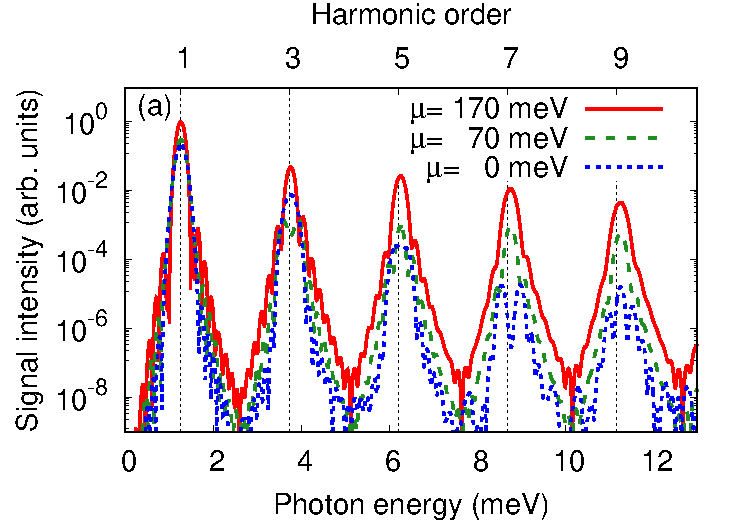
\includegraphics[width=0.8\linewidth]{pic/hhg_mu.pdf}
\caption{\label{fig:hhg_mu} 
Computed harmonic spectra $I_{\mathrm{HHG}}(\omega)$ with Eq.~(\ref{eqn:spectrum}) for different
chemical potentials, $\mu = 0$, $70$ and $170$~meV.}
\end{figure}

In Figure~\ref{fig:hhg_mu}, we present the computed HHG spectra, denoted as $I_{\mathrm{HHG}}(\omega)$, corresponding to different chemical potentials $\mu$. Each chemical potential yields distinct harmonic peaks, and a noticeable trend emerges: the intensities of the emitted harmonics systematically increase with the rise in the chemical potential. This observation aligns with findings from a recent experiment \cite{kovalev2021electrical}, where an analogous increase in emitted harmonic intensity was noted with an elevation in gate voltage.

The results presented here echo the interpretations from prior research, such as \cite{mics2015thermodynamic}, where THz-induced high-order harmonic generation in graphene was elucidated through a thermodynamic framework. In contrast, our current study aims to advance the understanding of these THz-induced nonlinear phenomena by incorporating a comprehensive microscopic perspective. Specifically, we delve into the nonequilibrium nature of electron dynamics to refine our description of light-matter interactions and provide a more nuanced interpretation of the observed trends in high-order harmonic spectra with varying chemical potentials.

Following the electron dynamics calculations under THz fields, our findings reveal that the emitted harmonics experience enhancement with an increase in chemical potential. This theoretical insight aligns with recent experimental observations, where high-order harmonic generation is similarly enhanced through the application of a gate bias voltage \cite{kovalev2021electrical}.
%%%%%%%%%%%%%%%%%%%%%%%%%%%%%%%%%%%%%%%%%%%%%%%%%%%%%%%%%%%%%%%%%%%%%%%%%%%%%%%%%%%%%%%%%%%%%%%%%%%%%%%%%%%%%%%%%%%%%%%%%%%%%%%%%%
\section{Quasi-static Approximation}
%%%%%%%%%%%%%%%%%%%%%%%%%%%%%%%%%%%%%%%%%%%%%%%%%%%%%%%%%%%%%%%%%%%%%%%%%%%%%%%%%%%%%%%%%%%%%%%%%%%%%%%%%%%%%%%%%%%%%%%%%%%%%%%%%%
 Subsequently, we introduce a quasi-static approximation to dissect the THz-induced electron dynamics, facilitating a reexamination of the nonlinear electric transport and the field-induced transparency phenomena inherent to graphene \cite{sato2021nonlinear}.
 In our analysis, we make the assumption that the variation of the THz field is sufficiently slow, allowing the electronic system to be effectively characterized by a nonequilibrium steady state at each point in time. This assumption holds true under the equilibrium established between the field-induced excitation and relaxation processes. Its accuracy is particularly pronounced when the mean frequency of the THz field is significantly smaller than the intrinsic relaxation rates, denoted as $1/T_1$ and $1/T_2$.

For practical considerations within the quasi-static approximation, we initiate our analysis by evaluating the electric current of a nonequilibrium steady state under a static electric field, represented as $\vecb E(t)=E_0 \vecb e_x$. The corresponding expression is given by:

\begin{align}
\vecb J_S(E_0) = \lim_{t\rightarrow \infty}\frac{2}{(2\pi)^2}\int d\vecb k \mathrm{Tr}\left[\hat{\boldsymbol{J}}{\boldsymbol{k}}(t)\rho{\boldsymbol{k}}(t)\right].
\label{eq:steady-current}
\end{align}

In this equation, the electron dynamics are computed under a static field, $\vecb{A}(t)=-E_0
\vecb{e}_x t$. Over time, the electronic system attains a nonequilibrium steady state as a result
of the equilibrium between field-induced excitation and relaxation processes. 

Within the quasi-static approximation, we substitute the instantaneous electric field in the induced current $\vecb J(t)$ with the steady current $\vecb J_S(E_0)$ from Eq.~(\ref{eq:steady-current}), resulting in the approximation:

\begin{align}
\vecb J(t)\approx \vecb J_S\left( \vecb E(t) \right).
\label{eq:appendix-steady-current}
\end{align}

To assess the validity of this approximation, we first evaluate the steady current in
Eq.(\ref{eq:steady-current}) for various field strengths. For practical computations, we analyze
the electron dynamics under a static electric field, denoted as $\vecb E_0=E_0\vecb e_x$.
Figure\ref{fig:steady} depicts the computed current as a function of time under a static field. In this simulation, the chemical potential $\mu$ is set to $170$~meV, and the field strength $E_0$ is established at $8.5$~MV/m. The initial state at $t=0$ corresponds to the thermal equilibrium state.
\begin{figure}[htb]
    \centering
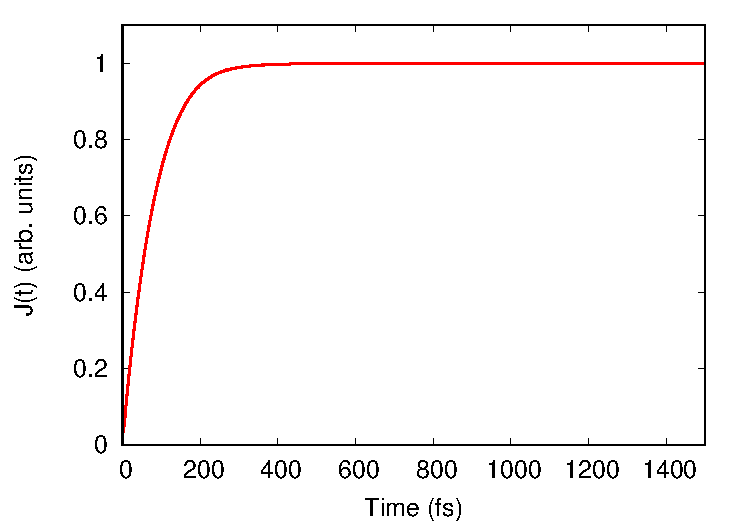
\includegraphics[width=0.8\linewidth]{pic/steady_current_appendix.pdf}
\caption{\label{fig:steady}
Electric current in graphene under a static electric field, $E_0=8.5$~MV/m.}
\end{figure}

As observed in Fig.\ref{fig:steady}, the application of the electric field induces an electric current at $t=0$, and it steadily approaches the steady-state value, denoted as $\vecb J_S(E_0)$. This observation confirms that the electronic system, evolving under Eq.(\ref{eqn:masterequation}) with a static electric field, eventually reaches a nonequilibrium steady state after a sufficiently extended period of time propagation. This validation supports the reliability of the quasi-static approximation in capturing the nonequilibrium dynamics induced by a slowly varying electric field.
\begin{figure}[htb]
    \centering
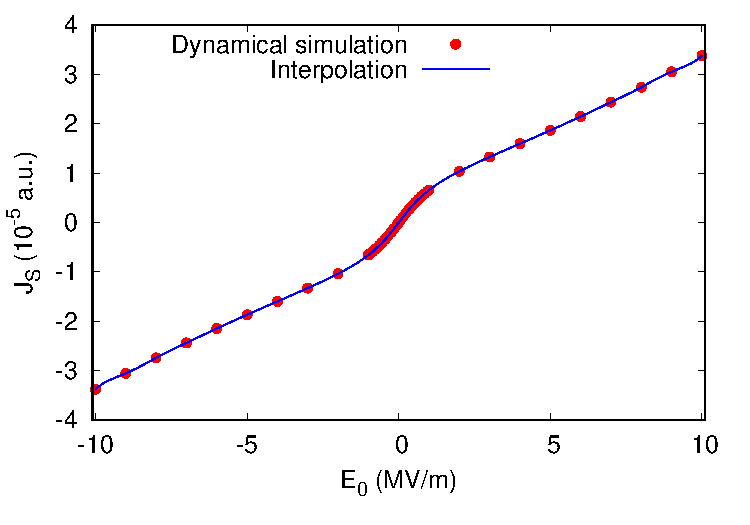
\includegraphics[width=0.8\linewidth]{pic/jsteady_interpolate.pdf}
\caption{\label{fig:insert} 
Steady current $\vecb J_S(E_0)$ as a function of field strength $E_0$. The results of the fully dynamical calculation are showns as the red points, while the interpolated result is shown as the blue-solid line.}
\end{figure}

In our iterative simulations, we systematically vary the field strength $E_0$ and assess the resulting values of the steady current. Denoting the $k$th set of employed field strength and evaluated current as $E_k$ and $\vecb J_k$ respectively, we represent the computed steady current $\vecb J_k$ as red points in Figure~\ref{fig:insert} against the applied field strength $E_k$. To construct a continuous function $\vecb J_S(E_0)$ from the discrete data points ${E_k, \vecb J_k}$ in Figure~\ref{fig:insert}, we adopt a two-step interpolation procedure.

\begin{figure}[htb]
    \centering
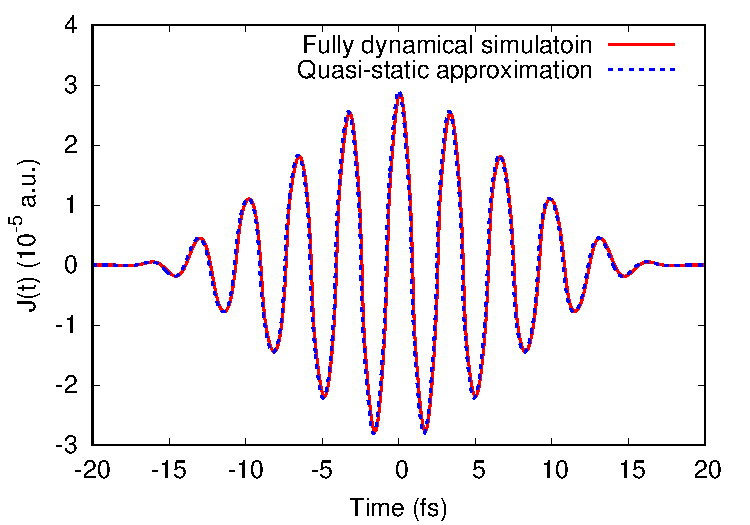
\includegraphics[width=0.8\linewidth]{pic/current_comparison_appendix.pdf}
\caption{\label{fig:current} Comparison of the THz-induced current computed with the fully dynamical calculation and the quasi-static approximation.}
\end{figure}

In the initial step of constructing the continuous function, we employ a polynomial regression with the following odd function:

\begin{align}
\vecb{J}_{\mathrm{polynomials }}(E_0)= \sum\limits{j=0}^{4} \vecb e_x \alpha^{(2j+1)} E^{2j+1}_0,
\label{eq:appendix-polynomial}
\end{align}

where $\alpha^{(j)}$ represents optimization parameters. These parameters are fine-tuned to ensure that the polynomial function $\vecb{J}_{\mathrm{polynomials }}(E_0)$ effectively reproduces the discrete points ${E_k, \vecb J_k}$ in Figure~\ref{fig:insert}.

Moving on to the second step, we aim to refine the discrepancy between the discrete points in Figure~\ref{fig:insert} and the polynomial function $\vecb{J}_{\mathrm{polynomials }}(E_0)$. To achieve this, we define the residual error of the polynomial regression as:

\begin{align}
\Delta \vecb{J}_k=\vecb{J}_{k}-\vecb{J}_{\mathrm{polynomials}}(E_k).
\end{align}

Subsequently, we apply spline interpolation to the data points ${E_k, \Delta \vecb{J}k}$, denoting the interpolated function as $\Delta \vecb{J}{\mathrm{spline}}(E_0)$. Finally, we approximate the continuous function, $\vecb J_S(E_0)$, as:

\begin{align}
\vecb J_S(E_0)\approx \vecb{J}_{\mathrm{polynomials }}(E_0)+\Delta \vecb{J}_{\mathrm{spline}}(E_0).
\label{eqn:approx}
\end{align}

\begin{figure}[htb]
    \centering
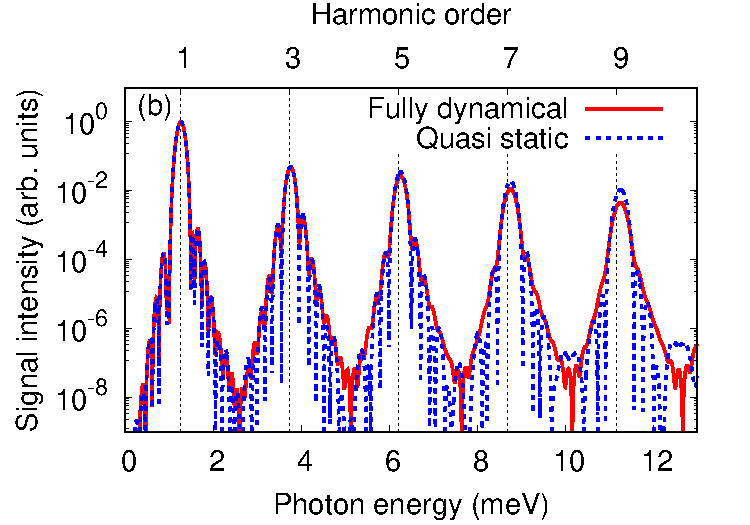
\includegraphics[width=0.8\linewidth]{pic/hhg_qstatic.pdf}
\caption{\label{fig:hhg_qstatic} 
Comparison of the HHG spectra computed with the fully dynamical simulations in Sec.~\ref{subsec:dynamical_simulation} and the quasi-static approximation Sec.~\ref{subsec:quasi-static}. Here, the chemical potential is set to $\mu =170$~meV.}
\end{figure}

Utilizing the approximated function in Eq.(\ref{eqn:approx}), we evaluate the THz-induced electric
current with the quasi-static approximation, Eq.(\ref{eq:appendix-steady-current}).
The relationship between current and field as expressed in Eq.~(\ref{eq:steady-current}), we approximate the field-induced current $\vecb J(t)$ by the steady-state current, where the instantaneous electric field is denoted as $\vecb E(t)$, leading to the approximation $\vecb J(t)\approx \vecb J_S\left( \vecb E(t) \right)$.
Figure~\ref{fig:current} showcases the computed current as a function of time with the quasi-static
approximation. To facilitate comparison, the result of the fully dynamical calculation is also
presented. Applying a Fourier transform to the obtained current in Figure~\ref{fig:current} yields
the high-order harmonic generation (HHG) spectra depicted in Figure~\ref{fig:hhg_qstatic}.

To gauge the accuracy of the quasi-static approximation, we computed the high-order harmonic
generation spectrum $I_{\mathrm{HHG}}(\omega)$ using the approximated current, $\vecb J_S\left(
\vecb E(t) \right)$. Figure~\ref{fig:hhg_qstatic} illustrates the computed spectrum $I_{\mathrm{HHG}}(\omega)$ with the quasi-static approximation, with $\mu$ set to $170$~meV. For reference, the corresponding result from the fully dynamical calculation is also presented. As evident from the figure, the quasi-static approximation faithfully reproduces the results obtained from the fully dynamical calculation. Thus, we confirm that the quasi-static approximation adeptly captures the electron dynamics in graphene under THz fields. This observation suggests that the microscopic mechanism of THz-induced high-order harmonic generation (HHG) in graphene can be effectively elucidated based on the nonequilibrium steady state, considering the delicate balance between field-induced excitation and relaxation. It is worth noting that the accuracy of the quasi-static approximation diminishes for higher-order harmonics due to the rapid dynamics that cannot be adequately captured by the quasi-static picture.

We have validated that the THz-induced high-order harmonic generation in graphene is effectively captured by the quasi-static approximation, highlighting the relevance of the nonequilibrium steady-state in portraying essential aspects of THz-induced electron dynamics. A detailed microscopic analysis has been conducted to examine the significance of the intraband current and the population distribution within the Brillouin zone in this steady-state.
%%%%%%%%%%%%%%%%%%%%%%%%%%%%%%%%%%%%%%%%%%%%%%%%%%%%%%%%%%%%%%%%%%%%%%%%%%%%%%%%%%%%%%%%%%%%%%%%%%%%%%%%%%%%%%%%%%%%%%%%%%%%%%%%%%
\section{Nonlinear Charge Transport in Nonequilibrium Steady-state}
%%%%%%%%%%%%%%%%%%%%%%%%%%%%%%%%%%%%%%%%%%%%%%%%%%%%%%%%%%%%%%%%%%%%%%%%%%%%%%%%%%%%%%%%%%%%%%%%%%%%%%%%%%%%%%%%%%%%%%%%%%%%%%%%%%
To provide a broader context, we juxtapose the nonequilibrium steady-state achieved within the quasi-static framework with insights garnered from a recently developed thermodynamic model \cite{mics2015thermodynamic}. This comparative analysis aims to elucidate the nonequilibrium mechanisms governing nonlinear optical and transport phenomena within graphene in the THz regime. By contrasting the quasi-static nonequilibrium picture with the thermodynamic model, we endeavor to unravel the underlying dynamics driving the intricate interplay between electron behavior and external THz fields in graphene systems.
We then study the nonlinear electric conductivity in a static regime in order to develop
microscopic insight into the THz-induced HHG. For this purpose, we first define the intraband
component of the steady-state current in Eq.~(\ref{eq:steady-current}).

Next, we proceed to evaluate the effective conductivities using both the total steady current
$\vecb J_S(E_0)$ and the intraband component $\vecb J^{\mathrm{intra}}_S(E_0)$. The effective total
and intraband conductivities are computed as follows:

\begin{align}
\sigma(E_0)=\frac{\vecb e_x\cdot \vecb J_S(E_0)}{E_0} \quad,\\
\quad \sigma^{\mathrm{intra}}(E_0)=\frac{\vecb e_x\cdot \vecb J^{\mathrm{intra}}_S(E_0)}{E_0}.
\end{align}

Figure~\ref{fig:conductivity} illustrates the computed effective conductivities, $\sigma(E_0)$ and $\sigma^{\mathrm{intra}}(E_0)$, as a function of the applied field strength $E_0$ for different chemical potentials $\mu$. In this figure, the conductivities $\sigma(E_0)$ obtained from the total steady current $\vecb J_S(E_0)$ align well with those derived from the intraband current $ \vecb J^{\mathrm{intra}}_S(E_0)$ across all investigated field strengths $E_0$ and chemical potentials $\mu$. This observation implies that the charge transport in graphene under static and THz fields is predominantly governed by the intraband current. The intraband current is described by the product of the band group velocity and the band population in the Brillouin zone.

\begin{figure}[htb]
    \centering
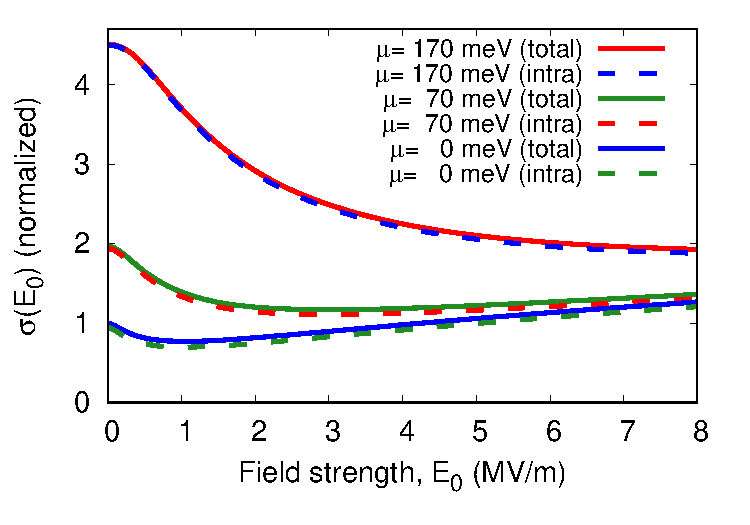
\includegraphics[width=0.8 \linewidth]{pic/sigma_vs_E0.pdf}
\caption{\label{fig:conductivity} 
Nonlinear effective conductivities of graphene as a function of the static field strength $E_0$ evaluated with the total currents (solid lines) and intraband currents (dashed lines) for different values of the chemical potential, $\mu = 0$, $70$ and $170$~meV.}
\end{figure}

In Fig.~\ref{fig:conductivity}, the effective conductivities, $\sigma(E_0)$, exhibit an initial
reduction across all investigated chemical potentials $\mu$ as the field strength increases from
zero. This reduction in conductivity aligns with the field-induced transparency phenomenon observed
in graphene \cite{sato2021nonlinear}, as the conductivity $\sigma(E_0)$ is directly related to
photoabsorption via Joule heating, given by:
\begin{align}
    E_{\mathrm{Joule}}=\vecb E_0 \cdot \vecb J_S(E_0)=\sigma(E_0)E^2_0
\end{align}
    As the field strength continues to increase, graphene with relatively small chemical potentials (e.g., $\mu=0$ or $70$~meV) exhibits an increase in conductivity, while graphene with a relatively large chemical potential (e.g., $\mu=170$~meV) continues to show a reduction in conductivity. These trends are consistent with a previous theoretical study on nonlinear transport in graphene using the linear band approximation \cite{sato2021nonlinear}:
    \begin{align}
H_{\vecb k}=v_F\left (\sigma_x k_x +\sigma_y k_y \right)
\end{align}
Given that the present work employs a more comprehensive electronic structure throughout the full Brillouin zone based on the tight-binding model, it serves as a validation of the low-energy Hamiltonian approximation for the graphene bandstructure used in the previous work. In the previous study \cite{sato2021nonlinear}, the decrease in effective conductivity was attributed to the dispersion of the population imbalance in the Brillouin zone, while the increase in conductivity was linked to additional carrier injection through the Zener tunneling mechanism. These interpretations naturally apply to the results obtained in the present study, further confirming the robustness and applicability of the previously proposed mechanisms.
 \begin{figure}[htb]
    \centering
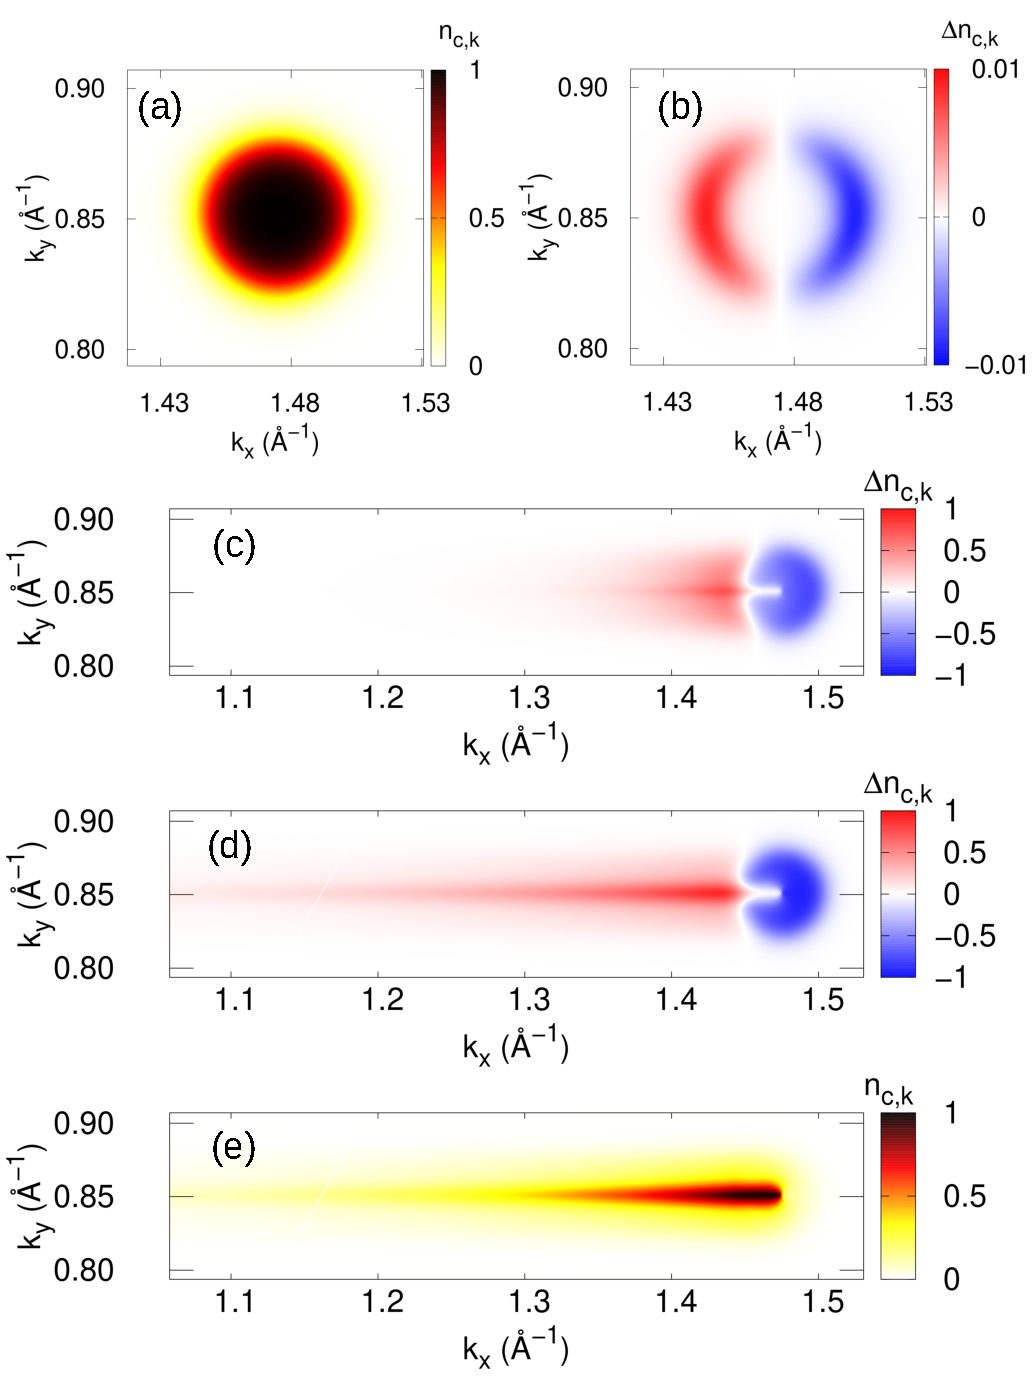
\includegraphics[width=1.0\linewidth]{pic/pop_fig.pdf}
\caption{\label{fig:pop_f}
(a) The equlibrium population distribution in the conduction band $f^{\mathrm{FD}}(\epsilon_{c,\vecb k})$. (b-d) The field induced conduction population change for different field strengths, (b) $0.01$~MV/m, (c) $3$~MV/m, and (d) $10$~MV/m. (e) The population distribution in the conduction band in the nonequilibrium steady-state under a static field, $E_0=10$~MV/m.}
\end{figure}

Given the aptitude of the quasi-static approximation in accurately delineating THz-induced electron
dynamics, the interpretation of THz-induced High-Order Harmonic Generation (HHG) finds its
foundation in the effective conductivities, as portrayed in Fig.~\ref{fig:conductivity}. Should the
conductivity $\sigma(E_0)$ remain unswayed by the field strength $E_0$, the induced current
maintains linear proportionality to the field strength, thereby precluding the generation of
harmonics. Consequently, within the quasi-static framework, the emergence of harmonics stems from
the nonlinearity inherent in the current $\vecb J_S(E_0)$ and the field-strength-dependent
conductivity $\sigma(E_0)$.

Examining Fig.\ref{fig:conductivity}, it becomes evident that the conductivity exhibits heightened sensitivity to the field strength, particularly accentuated for larger chemical potentials. This accentuated dependence manifests as a pronounced reduction in conductivity with increasing field strength. This observation underpins the elucidation of the heightened HHG in Fig.\ref{fig:hhg_mu} accompanying a shift in chemical potential—attributed to the significant reduction in conductivity coincident with the amplified field strength.

In prior investigations \cite{hafez2018extremely,kovalev2021electrical}, the interpretation of THz-induced HHG in graphene was anchored in the reduction of conductivity, albeit within the framework of the thermodynamic model \cite{mics2015thermodynamic}. To unravel the influence of nonequilibrium dynamics in the steady state, we shall delve into the interrelation between the two models—the nonequilibrium steady-state model and the thermodynamic model—in the forthcoming section, Sec.~\ref{sec:thermo}.

Moving to the intraband current articulated in Eq.(\ref{eqn:intra-steady-current}), it is crucial to recognize its composition—encompassing the product of band velocity and population. Given the inherent invariance of band velocity under the presence of electric fields as an intrinsic material property, the crux of THz-induced current generation lies in the field-induced modulation of population. Furthermore, as expounded earlier, the THz-induced current is predominantly governed by the intraband component. For an intricate understanding of the THz-induced current at a microscopic level, we shall undertake an analysis of the population distribution within the Brillouin zone under the influence of the field. Figure\ref{fig:pop_f}~(a) delineates the equilibrium population distribution in the conduction band, denoted as $f^{\mathrm{FD}}(\epsilon_{c,\vecb k})$, around a Dirac point (K point) in graphene, specifically at $\vecb k =\frac{2\pi}{\sqrt{3}a}\left(1, \frac{1}{\sqrt{3}}\right)$. Here, the chemical potential $\mu$ is established at $170$~meV. The equilibrium population exhibits a circular symmetry around the Dirac point, reflecting the partial filling of the Dirac cone by doped electrons.

We define the field-induced alteration in conduction population within a nonequilibrium steady
state as:
\begin{align}
    \Delta n_{c,\vecb{k}}= \left [n_{c, \vecb{k}'+e\vecb{A}(t)/\hbar}(t)- f^{FD}(\epsilon_{c,\vecb{k}'+e\vecb A (t)/\hbar})\right ]_{\vecb k'+e\vecb A(t)/\hbar =\vecb k}
\end{align}
Figures~\ref{fig:pop_f}~(b-d) showcase the field-induced conduction population $\Delta n{c,\vecb{k}}$ for varying field strengths: (b)~$0.01$MV/m, (c)$3$MV/m, and (d)$10$~MV/m.

As illustrated in Fig.\ref{fig:pop_f}(b), the field-induced population modulation emerges along the
ring-shaped contour defined by the single-particle energy $\epsilon_{b\vecb k}$ and the Fermi
energy $\epsilon_{\mathrm F}=\mu\big |_{T_e=0}$ as $\epsilon_{b\vecb k}=\epsilon_{\mathrm F}$,
specifically where $\epsilon_{b \vecb k}=\epsilon_{\mathrm F}$. The modulation occurs in proximity to the Fermi energy due to the mild field excitation, and the ring structure derives from the circular symmetry inherent in the Dirac cone. In the weak field regime, the augmentation and reduction in conduction population $\Delta n_{c,\vecb{k}}$ exhibit symmetric distribution along the field direction ($x$-axis). Conversely, in the strong-field regime, the distribution becomes non-symmetric, as evident in Figs.\ref{fig:pop_f}(c) and (d). Here, the red-colored region signifies an expanded range on the left side of the Dirac point, where population increase occurs, while the blue-colored region indicates a more confined area on the right side marked by population decrease. The pronounced elongation of the population increase along the field direction may be construed as a consequence of the field-induced intraband acceleration within the Brillouin zone. Simultaneously, the localized population decrease around the Dirac point, as observed in Fig.\ref{fig:pop_f}(a), can be attributed to the field-induced displacement of initially localized electrons encircling the Dirac point.

In the preceding study \cite{sato2021nonlinear}, the decrease in conductivity was elucidated as the
saturation of population imbalance surrounding the Dirac point. To scrutinize this interpretation,
we present the conduction population distribution:
\begin{align}
n_{c,\vecb k'+e\vecb A(t)/\hbar}\big |_{\vecb k'+e\vecb A(t)/\hbar=\vecb k}
    \end{align}
in lieu of the population change $\Delta n{c,\vecb{k}}$ in Fig.\ref{fig:pop_f}(e), with the field strength $E_0$ set to $10$MV/m. It is noteworthy that the summation of the density in Fig.\ref{fig:pop_f}(a) and the density change in Fig.\ref{fig:pop_f}(d) corresponds to the density in Fig.\ref{fig:pop_f}~(e).

Examining Fig.\ref{fig:pop_f}(e), a discernible shift in the conduction population from the right to the left side of the Dirac cone is evident. This observation indicates that the population imbalance encircling the Dirac cone is already near its maximum saturation point, where no further population can be transferred from the right side to the left side. Consequently, the population imbalance, a pivotal determinant of the intraband current, reaches saturation in the strong-field regime, precluding any substantial increase. This saturation, in turn, leads to the saturation of the intraband current—predominant in the nonequilibrium steady state—ultimately culminating in the observed reduction in conductivity within the strong-field regime.

Our investigation reveals a substantial decrease in the effective conductivity of graphene in the strong-field regime, attributed to the saturation of population imbalance within the Brillouin zone. This reduction aligns with the observed THz-induced transparency in graphene, as reported experimentally \cite{Hwang2013, Paul_2013, doi:10.1063/1.4902999} and theoretically investigated in prior studies \cite{sato2021nonlinear}. Furthermore, we establish that this diminished conductivity leads to nonlinear current behavior in the strong-field regime, culminating in high-order harmonic generation in graphene. Thus, the origin of high-order harmonic generation can be comprehended through the lens of saturation of population displacement within the Brillouin zone in the context of nonequilibrium electron dynamics.
%%%%%%%%%%%%%%%%%%%%%%%%%%%%%%%%%%%%%%%%%%%%%%%%%%%%%%%%%%%%%%%%%%%%%%%%%%%%%%%%%%%%%%%%%%%%%%%%%%%%%%%%%%%%%%%%%%%%%%%%%%%%%%%%%%
\section{Comparison with Thermodynamic Model \label{sec:thermo}}
%%%%%%%%%%%%%%%%%%%%%%%%%%%%%%%%%%%%%%%%%%%%%%%%%%%%%%%%%%%%%%%%%%%%%%%%%%%%%%%%%%%%%%%%%%%%%%%%%%%%%%%%%%%%%%%%%%%%%%%%%%%%%%%%%%
Having elucidated the microscopic intricacies of THz-induced High-Order Harmonic Generation (HHG) in graphene within the framework of the noneequilibrium steady-state, our focus now shifts to investigating the distinctive role played by the nonequilibrium nature of THz-induced electron dynamics. To accomplish this, we undertake a comparative analysis with the previously formulated thermodynamic model \cite{mics2015thermodynamic}. In contrast to the present nonequilibrium model, the thermodynamic model relies on the utilization of the thermal Fermi--Dirac distribution to delineate laser-excited electronic systems. This model operates under the assumption that electrons swiftly undergo thermalization, allowing them to be effectively treated as an equilibrium state characterized by a notably high electron temperature $T_e$.

\begin{figure}[htb]
    \centering
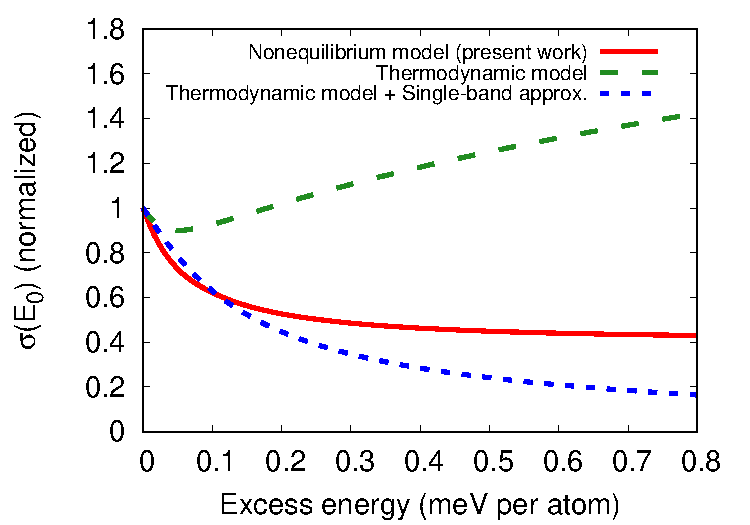
\includegraphics[width=0.8\linewidth]{pic/sigma_thermo.pdf}
\caption{\label{fig:compare} Computed effective conductivities are shown as a function of the excess energy. The results for the nonequilibrium steady-state (red-solid), the thermodynamic model (green-dashed), and the thermodynamic model plus the single-band approximation (blue-dotted) are shown.}
\end{figure}

Within the thermodynamic model, equilibrium states find characterization through the electron
temperature $T_e$, while in the developed nonequilibrium model, nonequilibrium steady-states are
intrinsically defined by the applied field strength $E_0$, devoid of any reliance on temperature
considerations. To ensure a equitable comparison between the two models, it becomes imperative to
establish a connection between the electron temperature $T_e$ and the field strength $E_0$. This connection is facilitated by the introduction of the field-induced excess energy for each model.

The total energy of the electronic system is formulated as:
\begin{eqnarray}
E_{\mathrm{tot}}(t)=\frac{2}{(2\pi)^2} \int d\vecb k \mathrm{Tr}\left[H_{\vecb k+ e\vecb A(t)/\hbar} \rho_{\vecb k}(t)\right].
\label{eqn:totalenergy}
\end{eqnarray}

Subsequently, the field-induced excess energy of the nonequilibrium steady-state is defined as
\begin{eqnarray}
\Delta E^\mathrm{NEQ}_{\mathrm{excess}}(E_0)=\lim_{t\rightarrow \infty} \left [E_{\mathrm{tot}}(t)
-E_{\mathrm{tot}}(-t) \right ],
\label{eq:excess-energy-neq}
\end{eqnarray}

Here, $\lim_{t\rightarrow \infty} E_{\mathrm{tot}}(t)$ corresponds to the total energy in the nonequilibrium steady-state under the presence of the field $E_0$, while $\lim_{t\rightarrow \infty} E_{\mathrm{tot}}(-t)$ corresponds to that of the equilibrium state without the field. Thus, the field-induced excess energy of the nonequilibrium model captures the energy difference between the nonequilibrium steady-state under an external field $E_0$ and the field-free equilibrium state.

In contrast, the field-induced excess energy of the thermodynamic model is defined as the energy difference between finite temperature states at $T_e$ and $300$K, the initial temperature of the present nonequilibrium model:
\begin{align}
\Delta E^\mathrm{TM}_{\mathrm{excess}}&=\sum_{b=v,c}\frac{2}{(2\pi)^2}\int d\vecb k
\epsilon_{b\vecb k} \nonumber \\
& \times \left [
f^{\mathrm{FD}}\left (\epsilon_{b\vecb k},T_e,\mu \right )
-f^{\mathrm{FD}}\left (\epsilon_{b\vecb k},T_e=300~\mathrm{K},\mu \right )
 \right ].
\label{eq:excess-energy-tm}
\end{align}

Therefore, $\Delta E^\mathrm{TM}_{\mathrm{excess}}$ is expressed as a function of the electron
temperature $T_e$.

By employing Eq.(\ref{eq:excess-energy-neq}) and Eq.(\ref{eq:excess-energy-tm}), we establish a link between the applied field strength $E_0$ characterizing the nonequilibrium steady-state and the electron temperature $T_e$ inherent to the thermodynamic model through the concept of excess energy. This connection enables a comparative analysis of the effective conductivity $\sigma(E_0)$ in the nonequilibrium steady-state and the linear conductivity of the thermodynamic model.

Figure~\ref{fig:compare} presents the conductivities of the nonequilibrium steady-state (depicted
by the red-solid line) and the thermodynamic model (represented by the green-dashed line). The
computations for the nonequilibrium steady-state consider a chemical potential $\mu$ set to
$170$~meV and an electron temperature $T_e$ in the relaxation operator set to $300$~K. In contrast,
the linear conductivity of the thermodynamic model is evaluated under the influence of a weak
field, ensuring the induced current aligns with a linear response. The results for the
thermodynamic model involve varying the electron temperature $T_e$ while maintaining the total
population constant, as expressed by:
\begin{align}
N_{\mathrm{tot}}=\frac{2}{(2\pi)^2}\sum_{b=v,c} \int d\vecb k f^{FD}(\epsilon_{b\vecb k},T_e,\mu),
\label{eq:tot-pop}
\end{align}
to the value at $T_e=300$~K and $\mu=170$~meV. Consequently, the chemical potential undergoes adjustments with changes in the electron temperature.

Figure~\ref{fig:compare} illustrates that the conductivity of the thermodynamic model (depicted by the green-dashed line) initially experiences a decline with an increase in the excess energy, followed by a notable upturn once the excess energy reaches a moderately large value. In contrast, the conductivity of the nonequilibrium steady-state (represented by the red-solid line) consistently diminishes with the escalation of the excess energy across the entire explored range. It's important to note that the conductivity of the nonequilibrium steady-state in Fig.\ref{fig:compare} aligns with that in Fig.\ref{fig:conductivity} when considering the converted $x$-axis. The fundamental contrast between the conductivities of the nonequilibrium steady-state and the thermodynamic model arises from the interband excitation influenced by temperature. In the thermodynamic model, thermal excitation propels electrons from the valence band to the conduction band, augmenting the effective carrier population and subsequently enhancing conductivity with elevated electron temperatures. In contrast, the nonequilibrium steady-state experiences a significant suppression of field-induced interband excitation due to Pauli blocking, mitigating the artificial rise in effective carrier population and the resultant boost in conductivity.

In their previous study \cite{mics2015thermodynamic}, the authors delved into the microscopic intricacies of THz-induced high-order harmonic generation and field-induced transparency in graphene using the thermodynamic model. Notably, the investigation adopted a single-band approximation in which only the conduction band was considered, while the valence band remained frozen. Surprisingly, this single-band approximation yielded better agreement with experimental results than the two-band approximation, where both valence and conduction bands were considered \cite{kovalev2021electrical}. Despite the intuitive expectation that the two-band approximation would offer greater accuracy, the results indicated that the single-band approximation provided a more accurate depiction within the thermodynamic model.

To elucidate the role of the single-band approximation in the thermodynamic model, we extended our comparison between the thermodynamic model and the nonequilibrium steady-state by incorporating the single-band approximation into our analysis. In this adaptation, we phenomenologically constrained the population in the valence band, while maintaining the use of the Fermi--Dirac distribution for the conduction band. This modification involved transforming the Fermi--Dirac distribution as follows:
\begin{align}
\tilde f^{\mathrm{MFD}}(\epsilon, T_e, \mu)=f^{\mathrm{FD}}(\epsilon, T_e, \mu)\Theta(\epsilon)+\Theta(-\epsilon),
\label{eq:mod-fd-dist}
\end{align}
where $\Theta(\epsilon)$ represents the Heaviside step function. By replacing the original Fermi--Dirac distribution (Eq.(\ref{eq:fd-dist})) with the modified version (Eq.(\ref{eq:mod-fd-dist})), we conducted a comparative analysis of conductivity with the thermodynamic model. The results of the thermodynamic model incorporating the single-band approximation are depicted by the blue-dotted line in Fig.~\ref{fig:compare}. Remarkably, this modified thermodynamic model effectively reproduces the conductivity trend observed in the nonequilibrium steady-state, showcasing a consistent monotonic decrease with an increase in excess energy.

This intriguing outcome suggests that the phenomenological freezing of the valence band in the single-band approximation curtails the artificial interband excitation in the thermodynamic model, leading to a more accurate portrayal of conductivity. In contrast, the nonequilibrium steady-state, based on a fully dynamical model, naturally captures the suppression of interband excitation, providing an accurate representation of electron dynamics in graphene under THz fields without resorting to the phenomenological freezing of the valence band.

Consequently, our findings indicate that the thermodynamic model exhibits an artificial augmentation of electric conductivity when subjected to intense THz fields, stemming from pronounced interband transitions between the valence and conduction bands. In alignment with prior work \cite{kovalev2021electrical}, we introduced a single-band approximation, freezing the valence band to mitigate this spurious interband excitation. Correspondingly, the computed conductivity in the thermodynamic framework, employing this single-band approximation, accurately reflects the anticipated decreasing trend under field irradiation. This trend aligns with experimental observations of the field-induced transparency of graphene \cite{Hwang2013, Paul_2013, doi:10.1063/1.4902999}. In contrast, the nonequilibrium model developed in this study effectively captures the diminishing trend in conductivity under field irradiation without the need for artificially freezing the valence band. This underscores the essential role of the nonequilibrium nature of electron dynamics in describing conductivity reduction under field irradiation and preventing spurious interband excitation, as evidenced in the comparison with the thermodynamic model.
